Úvod následující kapitoly stručně popisuje vznik a historii souborového sytému ZFS. Zbytek této kapitoly představuje strukturu ZFS, jeho základní stavební kameny a některé zajímavé principy, které tento souborový systém využívá. Pro názornost jsou v této kapitole uvedeny praktické ukázky příkazů sloužící k administraci ZFS.

\section{Úvod}
    %NICM MOC
    Souborový systém Zettabyte byl původně vyvinut společností Sun Microsystems a následně integrován do operačního systémů Solaris od stejnojmenné společnosti.
    Jak už to tak v dnešním světě bývá v roce 2010 společnost Oracle akvizicí společnosti Sun Microsystem získala operační systém Solaris a tím i vlastnictví ZFS \cite{suns}. V dnešní době tedy veškerý vývoj a podpora pro tyto systémy pochází právě od firmy Oracle \cite{guide}. Tyto dokumenty byly i hlavním zdrojem informací pro tuto bakalářskou práci.

    Systém byl původně navrhnut pro použití čistě v operační systém Solaris, s čímž se pojily i minimální požadavky pro provoz ZFS, které jsou představeny v následujícím seznamu \cite{requirements}.
    \begin{itemize}
      \item Architektura procesoru SPARC nebo x86
      \item Operační systém Solaris 10 6/06 nebo novější
      \item Minimální místo na disku 128 MB
      \item Minimální místo pro vytvoření poolu 64 MB
      \item Pro optimální výkon ZFS alespoň 1 GB operační paměti
    \end{itemize}

    Díky zveřejnění zdrojových kódů ZFS, došlo k adaptaci souborového systému i na jiné operační systémy než je Solaris. Hlavním příkladem jsou systémy s Linuxovým jádrem jako je například Debian, Fedora nebo CentOS.

\section{Struktura}
Většina tradičních souborových systémů se váže na jedno konkrétní zařízení. Aby bylo možné spojit se souborovým systémem více zařízení, byl zaveden takzvaný volume manager, který souborovému systému poskytoval iluzi, že se jedná o samostatné zařízení \cite{traditional}. Ve skutečnosti se pod touto vrstvou mohlo skrývat více disků, které se tváří jako jeden. ZFS se v tomto směru vydalo svojí vlastní cestou a zařízení agreguje do takzvaných poolů, které slouží jako datový základ pro jednotlivé souborové systémy.
\begin{figure}[!h]
    \caption{Agregace zařízení do poolu}
    \label{agregation}
    \centering
    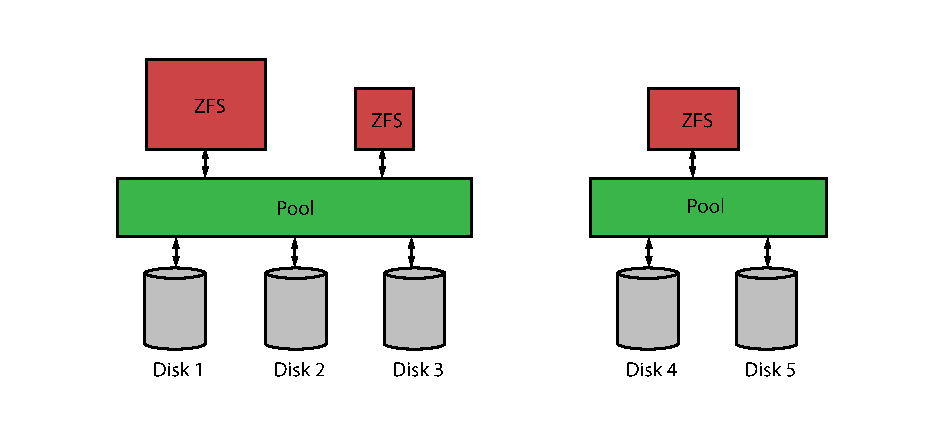
\includegraphics[scale=0.8]{agregation.pdf}
\end{figure}
\section{Pool}
Souborový systém ZFS se skládá ze dvou hlavních stavebních kamenů. Prvním z nich je takzvaný pool. V terminologii ZFS je to logické sdružení virtuálních zařízení, které popisuje rozložení a fyzické vlastnosti těchto zařízení \cite{terminology}. Pool je tedy spojení fyzických nebo virtuálních zařízení, která poskytuje základ pro souborové systémy ZFS.

Souborové systémy v ZFS se už neváží přímo na konkrétní fyzické zařízení, jak tomu bylo dříve, ale na pool jako celek. Historické spojení souborového systému s konkrétním fyzickým zařízením přinášela mnohá omezení. Například pokud jsme souborový systém chtěli rozšířit, museli jsme ho celý znovu vytvořit. Tato operace mohla být časově náročná, ale
v ZFS tomu tak není.
\subsection{Vlastnosti poolu}
ZFS si o každém vytvořeném poolu udržuje informace, které používá pro správu. Každý pool má seznam vlastností, které ho popisují a jednoznačně určují.
Hlavním identifikátorem poolu je jeho jméno. Toto jméno musí být v kontextu celého ZFS unikátní, protože se používá v příkazech manipulujících s daným poolem.

Vlastnosti můžeme rozdělit na dvě skupiny. Na jedné straně jsou statické vlastnosti, které popisují stav poolu a nedají se změnit přímo. Jsou takzvaně read-only. Pod tímto druhem vlastností si můžeme představit informace týkající se úložného prostoru jako je například velikost poolu, obsazená kapacita nebo volné místo. Velikost poolu nemůžeme změnit přímo nastavením odpovídající vlastnosti na jinou hodnotu, ale můžeme přidat do poolu další zdroj. ZFS tento krok rozpozná a související vlastnosti upraví.

Na druhé straně jsou vlastnosti, které můžeme měnit dynamicky. Některé z těchto vlastností se dají nastavovat pouze v okamžiku, kdy daný pool vytváříme nebo importujeme. Nastavit můžeme například vlastnost \emph{read-only}. Tato vlastnost zajistí, že od doby, kdy byla nastavena, lze z daného poolu data pouze číst a nikoliv data zapisovat. Další zajímavou vlastností je vlastnost \emph{bootfs}, která odkazuje na souborový systém uvnitř poolu, který slouží pro načítání operačního systému. Manuální nastavovaní této vlastnosti se nedoporučuje, protože špatné nastavení může vést k nenačtení operačního systému.

Pro stručnost jsem z následujícího příkazu, který administrátorovi zobrazuje dostupné informace o poolu, vybral pouze základní vlastnosti.
\begin{verbatim}
# zpool get all rpool
NAME   PROPERTY       VALUE                SOURCE
rpool  allocated      11.9G                -
rpool  bootfs         rpool/ROOT/solaris   local
rpool  capacity       38%                  -
rpool  dedupratio     1.19x                -
rpool  free           18.9G                -
rpool  health         ONLINE               -
rpool  readonly       off                  -
rpool  size           30.8G                -
\end{verbatim}

\subsection{Vytváření poolu}
Výše popsaný pool můžeme v systému ZFS kdykoli dynamicky vytvořit bez potřeby zásahu do operačního systému. Stačí když máme k dispozici potřebné zdroje (disk, partition, soubor) k vytvoření námi požadovaného poolu. Pokud máme požadované zdroje, stačí už jen vybrat unikátní jméno pro pool v kontextu ZFS a provést například následující příkaz.
\begin{verbatim}
$ zpool create tank c1t2d0 c2t1d0
\end{verbatim}
V případě dostupnosti disků c1t2d0 a c2t1d0, tento příkaz vytvoří pool jménem tank, do kterého tyto disky přiřadí. Výsledná velikost bude součtem velikostí těchto disků. Takto vytvořený pool neobsahuje žádnou redundanci a v případě selhání disku, může dojít ke ztrátě dat. Druhým typem, které ZFS podporuje, jsou redundandní pooly.
\subsection{Zrcadlení}
Prvním druhem redundadních poolů jsou ty, které obsahují virtuální zařízení \emph{mirror} nebo-li zdcadlení. Tento typ virtuálního zařízení můžeme pomocí ZFS vytvořit nad dvěma a více zařízeními. Uvnitř zařízení dochází k replikaci dat na všechny disky v zařízení. Výsledná kapacita virtuálního zařízení je tedy rovna kapacitě jednoho disku. Pokud zrcadlení vytvoříme nad třemi disky, nakonec budou data na všech třech discích stejná a v případě výpadku dvou z nich o data nepřijdeme. Jiná situace je samozřejmě v případě výpadku všech tří disků najednou. Zrcadlení nám v tomto případě nepomůže a všechny data ztratíme. Nicméně pravděpodobnost, že dojde k výpadku všech tří disků najednou, než stihneme alespoň jeden vyměnit, je malá.

Následující příkaz demonstruje jak vytvořit pool s redundantním zařízením \emph{mirror} o třech discích.
\begin{verbatim}
# zpool create Pool mirror c1t1d0 c1t2d0 c2t1d0
\end{verbatim}

\subsection{Raidz}
Druhým typem redundantních poolů, které ZFS umožňuje vytvářet, jsou pooly obsahující virtuální zařízení \emph{raidz}. Toto virtuální zařízení využívá jednoho nebo více paritních disků, které nám v případě výpadku nějakého disku umožní dopočítat ztracená data. Podle počtu paritních disků nám ZFS umožňuje vytvářet následující typy zařízení.
\begin{itemize}
  \item \emph{raidz1} - stripování s jedním paritním diskem
  \item \emph{raidz2} - stripování se dvěma paritními disky
  \item \emph{raidz3} - stripování se třemi paritními disky
\end{itemize}

Zápis dat na disk se provádí v pevně stanovených jednotkách tzv. stripech. Jeden stripe je rovnoměrně rozprostřen po všech datových discích virtuálního zařízení \emph{raidz}. Pokud bychom tedy zapisovali na disky soubor, který by měl přesně velikost stripu, bude soubor rovnoměrně rozprostřen na všech discích. Pokud by došlo k výpadku jednoho disku z virtuálního zařízení, dojde tím i k poškození určité části souboru a nebude možné tyto data přečíst. Pro tento účel se využívá paritních disků. Při zápisu stripu na disky se ze zapisovaných dat vypočte jedna hodnota, která se následně uloží na paritní disk. V případě výpadku jednoho disku z virtuálního zařízení, jsme schopni dopočítat chybějící data z hodnoty parity. Zvýšením počtu paritních disků jsme schopni dopočítat data při výpadku stejného počtu disků jako máme k dispozici paritních disků.
Pokud dojde v jednom okamžiku k výpadku více disků, než máme k dispozici paritních disků, dojde k nenávratné ztrátě dat.

Jelikož jsou data rovnoměrně rozmístěna na všechny disky ve virtuálním zařízení, můžeme při čtení dat využívat více disků najednou. Tím dokážeme docílit vyšší rychlosti čtení.

Následující příkaz ukazuje, jak jednoduše se dá v souborovém systému ZFS vytvořit redundantní pool typu \emph{raidz1}.
\begin{verbatim}
# zpool create Pool raidz1 c1t1d0 c1t2d0 c2t1d0 c2t2d0
\end{verbatim}

\subsection{Rozšiřování poolu}
Výhodou architektury poolů je možnost dynamického fyzických nebo virtuálních zařízení do poolu. Tím získáváme možnost dynamického rozšiřování kapacity celého poolu, která u tradičních souborových systému byla komplikovaná (nutnost použití VM) nebo nebyla dostupná vůbec. Souborové systémy v ZFS, které jsou vytvořené nad stejným poolem, sdílejí jeho prostředky, a proto při rozšíření kapacity tohoto poolu budou mít jeho souborové systémy k dispozici více místa pro ukládání dat.

V případě neredundantích poolů, které neobsahují virtuální zařízení typu \emph{mirror} nebo \emph{raidz}, můžeme pro rozšíření použít soubor, disk nebo část disku (partition). ZFS nám pro tento účel nabízí příkaz \verb|zfs add|, kterým můžeme dynamicky pool rozšiřovat.

Pokud pool obsahuje redundantní zařízení \emph{mirror} nebo \emph{raidz}, je doporučené pool rozšiřovat pouze o stejný typ zařízení. Pokud se do poolu typu \emph{mirror} pokusíme přidat virtuální zařízení \emph{raidz}, ZFS nás nám vypíše následující varovnou hlášku.
\begin{verbatim}
# zpool add Pool raidz1 c1t1d0 c1t2d0
mismatched replication level: pool uses mirror and vdev is raidz
\end{verbatim}

Využití souboru jako zdroje pro ZFS pool se v praxi téměř nevyužívá. Znamená to přidání další vrstvy mezi ZFS a samotný zdroj dat. Hlavní nevýhodou tohoto způsobu je značné zpomalení procesu čtení a zápisu dat, ale na druhou stranu se tato volba výborně hodí pro testování funkcí souborového systému ZFS.

\subsection{Zrušení poolu}
Stejně jako můžeme dynamicky pool vytvářet a rozšiřovat, můžeme pool i kdykoli zničit a uvolnit tak prostředky, které využíval. Tyto prostředky jsou ihned k dispozici a můžeme z nich vytvořit nový pool. Jelikož všechny souborové systémy vytvořené nad poolem sdílejí jeho prostředky, jsou tyto souborové systémy zničeny spolu s tímto poolem. Ke zničení poolu, který jsme dříve vytvořili, můžeme použít následující příkaz.
\begin{verbatim}
# zpool -r destroy tank
\end{verbatim}
Pokud v systému existuje pool jménem tank, příkaz ho zničí bez ohledu na to, kolik souborových systému nad tímto poolem bylo vytvořeno.

\section{Souborový systém}
Druhým ze stavebních kamenů ZFS jsou samotné souborové systémy. Jak bylo zmíněno v kapitole \ref{fs}, souborový systém je způsob organizace dat do souborů v datových úložištích.
Tradiční souborové systémy využívají k organizaci různých datových struktur. Souborový UFS využívá tzv. inodů, což je datová struktura držící atributy souboru a ukazatele na jednotlivé datové bloky \cite{ufs}. Souborový systém FAT k organizaci dat využívá tzv. file allocation table \cite{fat}. ZFS k tomuto účelu využívá stromové datové struktury, kterou znázorněna na obrázku \ref{structure}. Jedná se v podstatě o systém odkazů, který zároveň udržuje informace o souborech a adresářích. Bloky s daty se nacházejí v listech stromu.
\begin{figure}[!h]
    \caption{Struktura souborového systému ZFS}
    \label{structure}
    \centering
    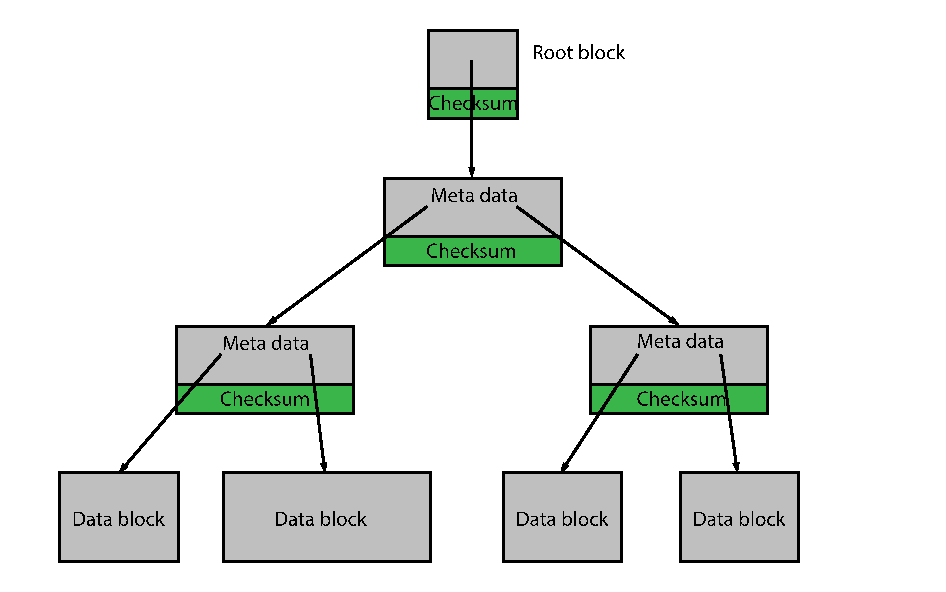
\includegraphics[scale=0.8]{zfsstructure.pdf}
\end{figure}

Tato stromová struktura přináší zajímavé výhody, které budou podrobněji popsány v dalších kapitolách.

\subsection{Hierarchie souborových systémů}
\label{hiararchy}
Jednou z vlastností ZFS je možnost hierarchického vnořování souborových systémů do sebe. Fakt, že samotný pool, jakožto zdroj místa pro souborové systémy, se chová jako samostatný souborový systém, tuto vlastnost dokazuje. Přesvědčit se o tom můžeme pomocí následujícího příkazu, kterému místo jména souborového systému předáme jméno poolu. Pokud příkaz proběhne dobře, vypíše základní informace o souborovém systému.
\begin{verbatim}
# zfs list rpool
NAME    USED  AVAIL  REFER  MOUNTPOINT
rpool  12.1G  18.2G  4.85M  /rpool
\end{verbatim}
Pokud by zmíněný souborový systém neexistoval, příkaz by vrátil chybovou hlášku.

Pool tedy tvoří hlavní uzel v této hierarchické posloupnosti a všechny souborové systémy vytvořené nad tímto poolem jsou jeho potomkem. V jednom poolu můžeme vytvořit více souborových systémů a také je do sebe můžeme libovolně vnořovat. Nejlépe si můžeme tuto hierarchii souborových systémů ukázat na obrázku \ref{fshierarchy}, kde můžeme vidět jak se do sebe jednotlivé souborové systémy vnořují.
\begin{figure}[h]
    \caption{Hierarchie souborových systémů ZFS}
    \label{fshierarchy}
    \centering
    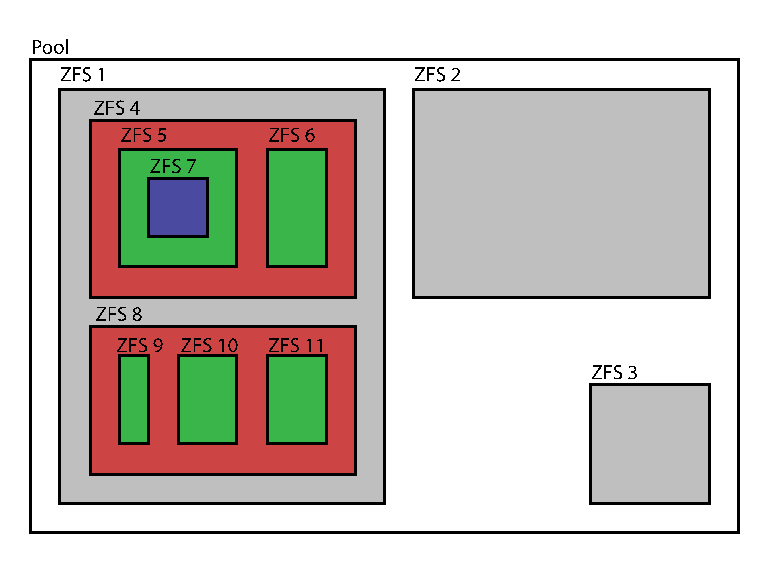
\includegraphics[scale=0.8]{hierarchy.pdf}
\end{figure}

\subsection{Vlastnosti souborového systému}
Stejně jako si ZFS udržuje u každého poolu jeho vlastnosti, udržuje si je také u každého souborového systému. Nastavováním těchto vlastností je administrátor schopen určit specifické chování konkrétního souborového systému. V kontextu ZFS má každý souborový systému jednoznačný identifikátor, který je odvozen z hierarchie souborových systémů. Skládá se z názvu systému a názvu jeho rodičů. Identifikátor by mohl vypadat následovně \emph{rpool/ROOT/solaris}.

Vlastnosti souborových systému můžeme rozdělit, stejně jako u vlastností poolu, na dvě kategorie. První kategorií jsou vlastnosti, které se dají pouze číst. Velkou část této skupiny tvoří vlastnosti popisující využití místa v souborovém systému. Příkladem může být místo spotřebováno vnořenými souborovými systémy nebo souborovým systémem samotným. V této skupině vlastností můžeme najít také datum vytvoření daného souborového systému nebo poměr deduplikace a komprese dat.

V druhé kategorii jsou vlastnosti, které může administrátor změnit za běhu nebo při vytváření souborových systémů. Stejně jako na úrovni poolu, tak i na úrovni souborového systému, můžeme nastavit vlastnost \emph{read-only}, která znemožní uživatelům zapisovat nebo měnit data v souborovém systému. Za povšimnutí dále stojí vlastnost \emph{exec}, která dovoluje v souborovém systému spouštět procesy.

Administrátor může jednoduše zapínat, vypínat či měnit vlastnosti souborového systému pomocí příkazu \verb|zfs set property=value rpool|, popřípadě si zobrazit seznam všech dostupných vlastností o souborovém systému pomocí \verb|zfs get all rpool|.

\subsection{Dědičnost}
Díky hierarchické struktuře se dá jednoduše zjistit, kdo je předkem daného souborového systému a kdo je jeho potomkem. Všechny nastavitelné vlastnosti, kromě kvót a rezervací, se dědí od rodičovského souborového systému. Pokud žádný rodič nemá vlastnost nastavenou explicitně, je použita standardní hodnota \cite{inheriting}.

Pokud chceme explicitně říci, aby některá vlastnost byla převzata od rodiče, můžeme použít příkaz \verb|zfs inherit property rpool|. Tento příkaz odnastaví danou vlastnost ze souborového systému a pokusí se převzít hodnotu z rodiče. Pokud v žádném z rodičů není hodnota nastavena explicitně, je použita standardní hodnota.
\subsection{Vytváření souborového systému}
\label{createfs}
Vytváření souborových systémů v ZFS je velice jednoduché. Jediné co potřebujeme k vytovření souborového systému je jednoznačný identifikátor. ZFS umožnuje vytvoření těchto systémů pomocí příkazu \verb|zfs create pool|, kde \emph{pool} je indentifikátor. Pokud neexistují všichni předci, je potřeba použít přepínač \verb|-p|, jinak příkaz selže.

Při vytváření je možné specifikovat, které vlastnosti daný souborový systém bude mít. Mimo jiné existují vlastnosti, které se dají nastavit pouze při vytváření. Po vytvoření souborového systému jsou tyto vlastnosti vedeny jako read-only a nedají se změnit. Jako příklad můžeme uvést vlastnost \emph{encryption}, která umožňuje šifrování souborového systému pomocí různých kryptografických funkcí. Pro využití této vlastnosti můžeme při vytváření poolu použít následující přepínač následující příkaz.
\begin{verbatim}
# zfs create -o enryption=on tank/pool/pool
\end{verbatim}
\subsection{Zrušení souborového systému}
Rušení souborových systému je v ZFS stejně snadné jako jejich vytváření. Je důležité mít na paměti, že zrušením souborového systému, který má nějaké potomky, zrušíme i všechny vnořené souborové systémy. Pro zrušení souborového systému pak již stačí použít příkaz \verb|zfs destroy| s příslušným identifikátorem, popřípadě přepínačem \verb|-r| pro zrušení všech potomků.
\subsection{Kvóty}
\label{quota}

Kvóty v ZFS umožňují administrátorovi spravovat limity souborových systémů týkajících se využitého místa. Tyto limity omezují možnosti využití dostupného místa v souborovém systému. Kvóty můžeme rozdělit do následujících kategorií podle toho, koho omezují.
\begin{itemize}
  \item Obecné - týkající se souborového systému
  \item Uživatelské - omezují jednotlivé uživatele
  \item Skupinové - omezují celé skupiny uživatelů
\end{itemize}

Obecné kvóty omezují místo, které může souborový systém využít jako celek. K tomuto účelu v ZFS slouží vlastnost \emph{quota}, která stanovuje limit místa, které může daný souborový systém využít. V tomto případě se do využitého místa započítává i místo spotřebované potomky \cite{quotas}. Pokud bychom chtěli omezit souborový systém bez ohledu na to kolik místa využijí jeho potomci, musíme použít vlastnost \emph{refquota}.
%% Rezervace

Vzhledem k faktu, že souborové systémy v jednom poolu sdílí diskové místo, ZFS přichází s vlastností \emph{reservation}. Tato vlastnost oproti kvótám garantuje souborovému systému diskové místo dané velikosti \cite{quotas}. Stejně jako v případě vlastnosti \emph{quota} je toto místo vyhrazeno pro souborový systém a všechny jeho potomky. Pokud bychom chtěli garantovat místo přímo souborovému systému, bez ohledu na to kolik místa využívají jeho potomci, musíme využít vlastnost \emph{refreservation}.

Jelikož vlastnosti \emph{quota} resp. \emph{refquota} a vlastnosti \emph{reservation} resp. \emph{refreservation} jsou vlastnostmi souborového systému, můžeme je nastavit stejně jako jakoukoli jinou vlastnost pomocí následujících příkazů.
\begin{verbatim}
# zfs set quota=10G rpool/export/home
# zfs set reservation=10G rpool/export/home
\end{verbatim}

Vztahy mezi vlastnostmi \emph{quota} a \emph{reservation} jsou vyznačeny na obrázku \ref{quotavsreserv}.
%% Obrázek
\begin{figure}[h]
    \caption{Vztahy mezi vlastnostmi \emph{quota} a \emph{reservation}}
    \label{quotavsreserv}
    \centering
    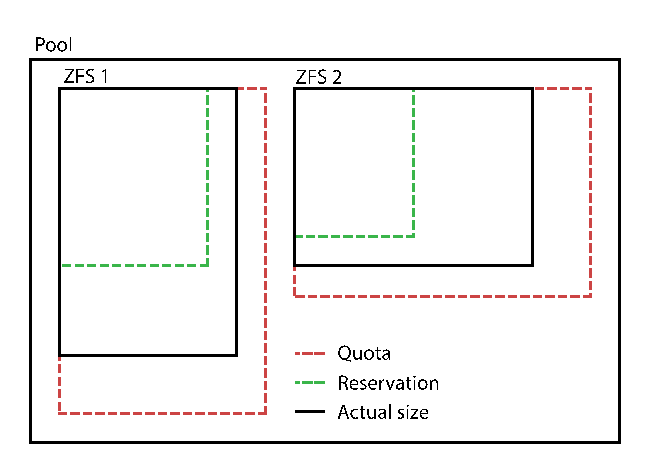
\includegraphics[scale=0.8]{quota.pdf}
\end{figure}
%% Uživatelské a skupinové kvóty

Další možností, jak omezit využití diskového místa, je pomocí uživatelských resp. skupinových kvót. Tyto kvóty limitují uživatele resp. skupinu v tom, kolik místa můžou v souborovém systému využít. Každý souborový systém má svůj vlastní \emph{userspace} resp. \emph{groupspace}, kde si udržuje informace o tom jaké mají limity jednotlivé skupiny resp. uživatelé.
Administrátor si může hodnoty uživatelských resp. skupinových kvót vypsat pomocí \verb|zfs userspace filesystem| resp. \verb|zfs groupspace filesystem|. Následující příkaz demonstruje, jak vypadá výpis uživatelských kvót pro domovský adresář.
\begin{verbatim}
# zfs userspace rpool/export/home/simactom
TYPE        NAME       USED  QUOTA  SOURCE
POSIX User  root      1.50K   none  default
POSIX User  simactom   641M   none  default
\end{verbatim}

Pokud se uživatel resp. skupina v seznamu nenachází nebo je u něj uvedena hodnota \emph{none}, uživatelské resp. skupinové kvóty se na něj nevztahují. Je-li v seznamu uvedena jiná hodnota, pak uživatel v daném souborovém systému nesmí překročit tuto hodnotu. Pokud by tuto hodnotu překročil, systém ho varuje a požadovanou akci neprovede. Přiřazení kvóty uživateli resp. skupině provedeme pomocí následujících příkazů
\begin{verbatim}
# zfs userquota@username=value filesystem
# zfs groupquota@username=value filesystem
\end{verbatim}

ZFS nabízí ještě vlastnost \emph{defaultuserquota} resp. \emph{defaultgroupquota}, kterou lze nastavit na určitou hodnotu. Tento limit se použije v případě, že hodnotu uživatelské resp. skupinové kvóty nastavíme na \emph{default}.
\section{Deduplikace}
\label{dedup}
Jednou z další vlastností, které ZFS nabízí, je deduplikace. Jak již z názvu vyplývá, jedná se o proces, který zabraňuje duplikaci stejných dat na disku a tím šetří i místo. Deduplikace se obecně dá rozdělit na následující úrovně.
\begin{itemize}
  \item Úroveň souborů
  \item Úroveň datavých bloků
  \item Úroveň bajtů
\end{itemize}

K identifikaci stejných dat se v ZFS využívá hešovácí funkce. Z porovnávaných dat jsou vytvořeny heše, které jsou následně porovnány. Pokud se heše rovnají a používáme kvalitní hešovací funkci, můžeme s velkou pravděpodobností říci, že jsou porovnávaná data opravdu totožná \cite{dedup}. Pokud je administrátor z nějakého důvodu stále nedůvěřivý, může u vlastnosti deduplikace nastavit hodnotu \emph{verify}, která zajistí celkové porovnání datových částí bajt po bajtu.

Deduplikace na úrovni souborů využívá nejméně systémových prostředků, protože se data hešují a porovnávají po velký částech. Na druhou stranu sebemenší změna v souboru vyžaduje přepočítání heše, který se již bude lišit od původního \cite{dedup}. Souborový systém pak rozpozná, že se soubory liší a uspořené místo bude zaplněno změněným souborem.

Deduplikace datových bloků vyžaduje oproti deduplikaci souborů vyšší využití systémových prostředků, ale na druhou stranu přináší v jistých situacích lepší úsporu místa \cite{dedup}.

V poslední řadě existuje deduplikace na úrovni bajtů, která je ze všech uvedených úrovní nejnáročnější na využití výpočetních prostředků. Tato možnost se používá jen ve speciálních případech.

ZFS z výše uvedených možností nabízí právě deduplikaci na úrovni datových bloků, protože tato jednotka deduplikace přináší nejvíce výhod v obecných případech použití \cite{dedup}. Na obrázku \ref{blockdedup} můžeme vidět porovnání souborového systému při zapnuté a vypnuté vlastnosti deduplikace.
\begin{figure}[!h]
    \caption{Ukázka deduplikce na úrovni datový bloků}
    \label{blockdedup}
    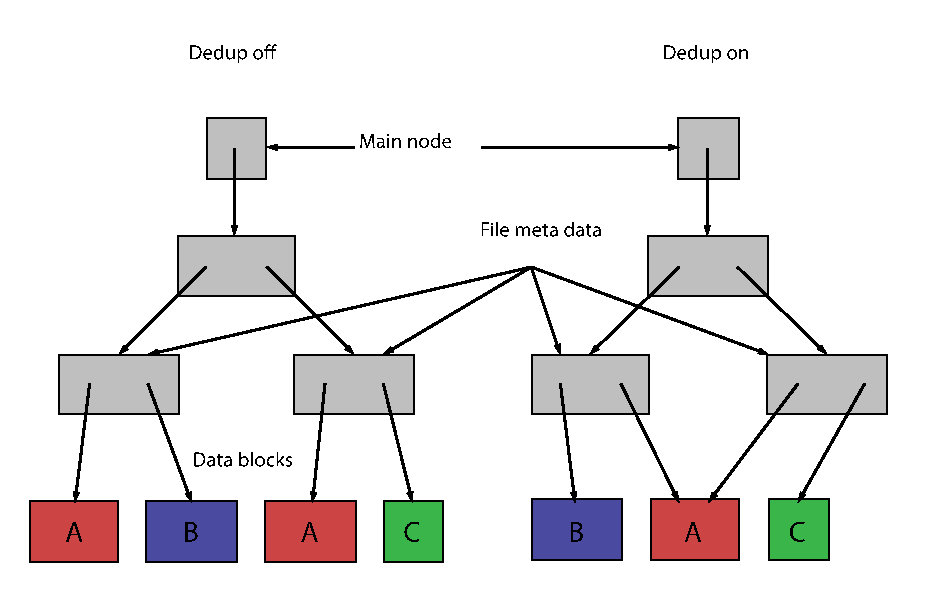
\includegraphics[scale=0.8]{dedup.pdf}
\end{figure}
\section{Konzistence}
\label{consitence}
Starší souborové systémy, jako například UFS, zapisují data přímo do bloku, který mění. To může v některých případech, jako je selhání systému nebo výpadek proudu, vést k nekonzistenci souborového systémů. V takovém případě je nutné celý souborový systém zkontrolovat například pomocí příkazu \verb|fsck|. Bohužel ani tento nástroj v některých případech nedokáže některé nekonzistence opravit \cite{transaction}.

Některé souborové systémy využívají tzv. žurnálů k pomoci s udržování konzistence dat. Žurnál je speciální záznam, kam se ukládají informace o tom, co a kde se bude měnit. Po provedení popisované akce se do žurnálu zapíše, že daná operace byla provedena. Když systém zkolabuje v jakémkoli kroku tohoto postupu, je možné ho při startu sytému dostat do konzistentního stavu. K tomuto účelu se opět využívá nástroj \verb|fsck|.

ZFS přichází s transakčním systémem a technikou copy on write. Tato technika zajišťuje neustálou konzistenci souborového systému i v okamžiku výpadku, a proto není třeba žurnálu. Data na disku nejsou nikdy přímo přepisována \cite{transaction}.

Transakce může vypadat následovně. Nejprve se vytvoří kopie bloků, které mají být změněny. V těchto kopiích dojde k vlastní změně dat, zatímco původní data jsou stále na disku a nejsou nijak změněna. Následně se provede kopie potřebných metadat, které se týkají měněných datových bloků. Tyto metadata jsou následně přepočítána podle nových datových bloků a konečně v poslední řadě se provede atomická operace, která připojí větev s novými resp. změněnými bloky do stromu souborového systémů.

Průběh transakce je naznačen na obrázku \ref{cow}. Celá transakce buď proběhla v pořádku nebo nebyla přijata vůbec. Pokud v průběhu transakce dojde k výpadku, celý souborový systém zůstává konzistentní, protože původní data jsou stále na disku a nemohla se provést atomická operace, která by připojila nové data.
\begin{figure}[h]
    \caption{Demostrace copy on write}
    \label{cow}
    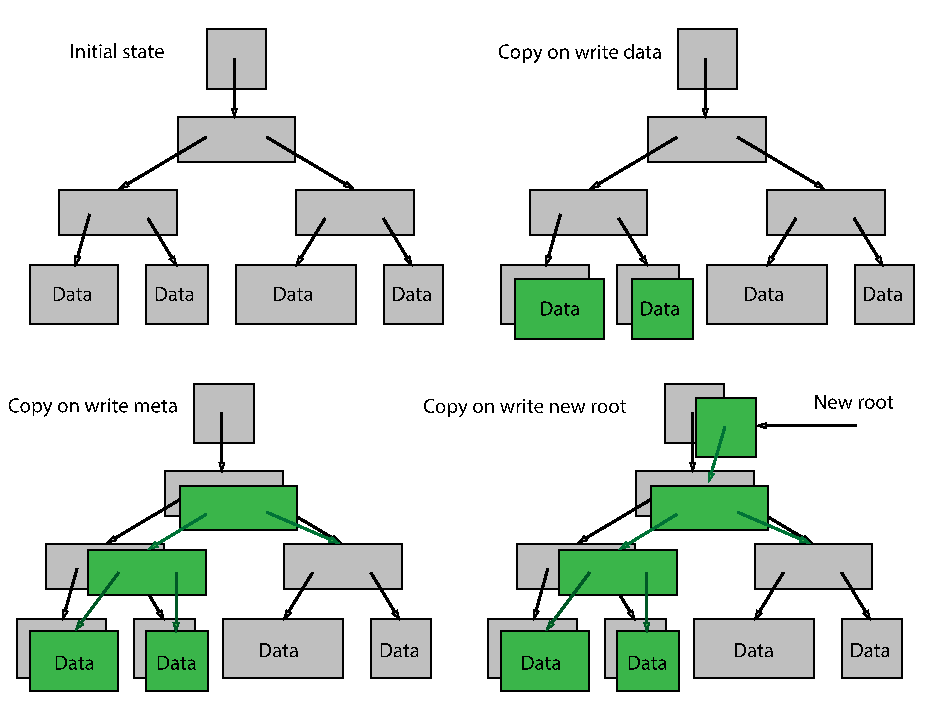
\includegraphics[scale=0.8]{cow.pdf}
\end{figure}
\section{Integrita dat}
\label{checksum}
Od souborového systému očekáváme, že při čtení dat z určitého datového bloku z disku, dostaneme data, která do tohoto bloku byla dříve zapsána. Pokud tomu tak není, měl by to souborový systém detekovat a vrátit chybu \cite{integrity1}.

Vlastnost neustálé konzistence souborového systému ZFS, zmíněná výše v kapitole \ref{consitence}, zajišťuje, že chybná data se v souborovém systému mohou vyskytnout jen chybou hardwaru \cite{integrity2}.

ZFS dokáže tyto chyby detekovat pomocí tzv. kontrolních součtů. Tyto součty vznikají a jsou přepočítávány při každé změně bloku v souborovém sytému. Jak jsme mohli vidět na obrázku \ref{structure}, součty nejsou uloženy v bloku, kterého se týkají, ale v bloku jemu nadřazeném. Při každém požadavku na čtení dojde k vypočítání kontrolního součtu na základě dat, které se v souborovém systému momentálně nachází a poté dojde k porovnání vypočteného součtu se součtem uloženým v nadřazeném bloku \cite{integrity1}. Tím ZFS dokáže rozhodnout zda je blok poškozený či nikoliv.

Díky těmto kontrolním součtům se souborový systém dokáže v určitých situacích sám opravovat. Tato situace nastává v případě, že blok, při jehož čtení došlo k chybě, je součástí redundantího virtuálního zařízení \emph{raidz} nebo \emph{mirror}. V tomto případě ZFS přečte datový blok i z replikovaného disku popřípadě sestaví blok pomocí parity a následně opraví chybný blok, při jehož čtení došlo k chybě. Aplikace dostane správná data i přes to, původně načtený datový blok byl poškozený.

Ačkoliv dochází k ověřování integrity dat automaticky při každém čtení z disku, je možné tento proces manuálně vyvolat a ověřit pomocí následující sekvence příkazů.
\begin{verbatim}
$ zpool scrub pool
$ zpool status pool
pool: pool
state: ONLINE
scan: scrub repaired 0 in 6s with 0 errors
\end{verbatim}

\section{Mountpoint}
\label{mountpoint}
Mounpoint je jednou ze základních vlastností všech souborových systémů. Je to vlastně cesta k bodu v adresářovém stromu operačního systému, kde má být daný souborový systém připojen.

Jelikož se ZFS snaží administrátorům maximálně ulehčit práci, stará se o automatické připojování souborových systémů sám. K účelům připojování souborových systémů v ZFS slouží jejich vlastnost \emph{mountpoint}, kde administrátor může specifikovat, kam se má daný souborový systém připojit. Pokud administrátor tuto vlastnost explicitně neurčí, je odvozena od vlastnosti rodičovského souborového systému.

Pro připojování souborových systémů ZFS se dají použít i tradiční nástroje \emph{mount} a \emph{umount}. V tradičních souborových systémech se pro automatické připojování používal soubor \emph{/etc/vsfstab}, kde administrátor specifikoval co a kam se má připojit. Operační systém po svém startu tento soubor zpracoval a vyznačené souborové systémy automaticky připojil.

Jak již bylo zmíněno ZFS proces automatického připojování provádí samo. Pokud by administrátor chtěl využívat tradičního připojování pomocí souboru \emph{/etc/vsfstab}, je možné nastavit vlastnost \emph{mountpoint} souborového systému na hodnotu \emph{legacy} \cite{mountpoint}. Tím administrátor řekne, že se o souborový systému bude starat sám a ZFS ho již automaticky připojovat nebude.
\section{Snapshot}
\label{snapshot}
ZFS snapshot je stav daného souborového systému v čase, kdy byl snapshot pořízen. Jedná se read-only instanci daného souborového systému \cite{snapshot}.

Díky stromové architektuře souborového systému ZFS je pořizování snapshotů velice elegantní a nenáročné. Pro vytvoření můžeme použít příkaz \verb|zfs snapshot filesystem@snapshot|, kde \emph{filesystem} je jméno souborového systémů, jehož stav chceme zachytit a \emph{snapshot} je pojmenování konkrétního stavu tohoto systému.

Po provedení příkazu k vytvoření snapshotu si ZFS zapamatuje odkaz na vrchol souborového systému, jehož snapshot tvoříme. Tento odkaz se stane hlavním kořenem snapshotu jakožto nového souborového systému. Jelikož snapshot je souborový systém určený pouze ke čtení, nemůžeme pomocí něj změnit data v aktivním souborovém systému. Po vytvoření snapshotu je jeho velikost nulová, protože se provedlo pouze zapamatování odkazu a nebyly vytvořeny žádné kopie. Pokud se ovšem data v aktivním souborovém systému změní, je nutné, aby snapshot stále odkazoval na stará data. Toho docílíme tak, že stará data zkopírujeme a zvětšíme tak velikost snapshotu \cite{snapshot}. Rozšiřování velikosti snapshotu tedy závisí na množství změněných dat od chvíle, kdy byl snapshot vytvořen. Proces vytváření snapshotu a rozšiřování jeho velikosti je názorně ukázán na obrázku \ref{snapshotproces}.
\begin{figure}[h]
    \caption{Vytváření snapshotu}
    \label{snapshotproces}
    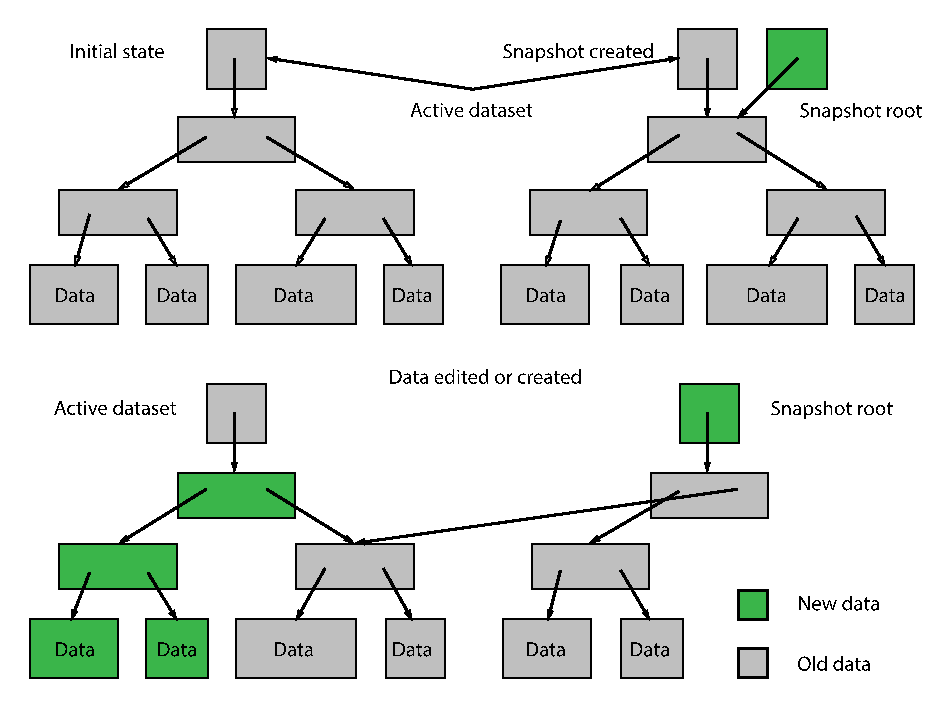
\includegraphics[scale=0.8]{snapshot.pdf}
\end{figure}

Rekurzivní tvorba snapshotů se provádí rychle pomocí jedné atomické operace. Snapshoty jsou vytvořeny naráz všechny dohromady nebo nejsou vytvořeny vůbec. Výhodou atomické operace je fakt, že data ve všech snapshotech jsou konzistentní vzhledem k jednomu časovému okamžiku \cite{snapshot}.

Snapshot pro souborový systém a všechny jeho potomky můžeme vytvořit pomocí následujícího příkazu.
\begin{verbatim}
# zfs snapshot -r rpool/export/home@snap
# zfs list -t snapshot -r rpool/export/home
NAME                             USED  AVAIL  REFER  MOUNTPOINT
rpool/export/home@snap              0      -    33K  -
rpool/export/home/simactom@snap     0      -   641M  -
\end{verbatim}
Druhý příkaz v pořadí ukazuje skutečnost, že snapshoty byly opravdu vytvořeny i pro všechny potomky daného souborového systému a že jejich velikost je opravdu nulová.

Snapshot se dá použít k navrácení souborového systému do stavu, v jakém se nacházel v okamžiku vytvoření snapshotu. Veškeré změny, které proběhly v souborovém systému od okamžiku vytvoření snapshotu budou smazány. K vyvolání tohoto procesu stačí použít příkaz \verb|zfs rollback snapshot |, kde \emph{snapshot} je celé jméno snapshotu. Jelikož se každý snapshot váže přímo s určitým souborovým systémem, není třeba zadávat jméno souborového systému, který chceme navrátit do původního stavu. 